\everymath{\displaystyle}
\documentclass{beamer}
% \documentclass[handout]{beamer}

%\usepackage[pdftex]{color,graphicx}
\usepackage{amsmath,amssymb,amsfonts}

\mode<presentation>
{
  % \usetheme{Darmstadt}
  % \usetheme[hideothersubsections]{Hannover}
  % \usetheme[hideothersubsections]{Goettingen}
  \usetheme[hideothersubsections, right]{Berkeley}

  \usecolortheme{seahorse}
  % \usecolortheme{dolphin}
  \usecolortheme{rose}
  % \usecolortheme{orchid}

  \useinnertheme[shadow]{rounded}

  \setbeamercovered{transparent}
  % or whatever (possibly just delete it)
}

\mode<handout>{
  \setbeamercolor{background canvas}{bg=black!5}
  \usepackage{pgfpages}
  \pgfpagesuselayout{4 on 1}[a4paper,border shrink=5mm, landscape]
}

\usepackage[brazilian]{babel}
% or whatever

% \usepackage[latin1]{inputenc}
\usepackage[utf8]{inputenc}
% or whatever

\usepackage{times}
%\usepackage[T1]{fontenc}
% Or whatever. Note that the encoding and the font should match. If T1
% does not look nice, try deleting the line with the fontenc.

% \usepackage[T1]{fontenc}
% \usepackage{lmodern}

\title%[] % (optional, use only with long paper titles)
{Bioestatística}

\subtitle
{Análise de Dados} % (optional)

\author%[] % (optional, use only with lots of authors)
{Felipe Figueiredo}% \and S.~Another\inst{2}}
% - Use the \inst{?} command only if the authors have different
%   affiliation.

\institute[INTO] % (optional, but mostly needed)
{Instituto Nacional de Traumatologia e Ortopedia
}
  % \inst{1}%
  % Department of Computer Science\\
  % University of Somewhere
  % \and
  % \inst{2}%
  % Department of Theoretical Philosophy\\
  % University of Elsewhere}
% - Use the \inst command only if there are several affiliations.
% - Keep it simple, no one is interested in your street address.

\date%[] % (optional)
{}

% \subject{Talks}
% This is only inserted into the PDF information catalog. Can be left
% out. 



% If you have a file called "university-logo-filename.xxx", where xxx
% is a graphic format that can be processed by latex or pdflatex,
% resp., then you can add a logo as follows:

\pgfdeclareimage[height=1.6cm]{university-logo}{../logo}
\logo{\pgfuseimage{university-logo}}



% Delete this, if you do not want the table of contents to pop up at
% the beginning of each subsection:
\AtBeginSubsection[]
%\AtBeginSection[]
{
  \begin{frame}<beamer>{\scriptsize Sumário}
    \tableofcontents[currentsection,currentsubsection]
  \end{frame}
}


% If you wish to uncover everything in a step-wise fashion, uncomment
% the following command: 

% \beamerdefaultoverlayspecification{<+->}

\usepackage[normalem]{ulem}

\begin{document}

\begin{frame}
  \titlepage
\end{frame}

\begin{frame}{Sumário}
  \tableofcontents
  % You might wish to add the option [pausesections]
\end{frame}


%% Template
% \section{}

% \subsection{}

% \begin{frame}{}
%   \begin{itemize}
%   \item 
%   \end{itemize}
% \end{frame}

% \begin{frame}
%   \begin{columns}
%     \begin{column}{5cm}
%     \end{column}
%     \begin{column}{5cm}
%     \end{column}
%   \end{columns}
% \end{frame}

% \begin{frame}{}
%   \includegraphics[height=0.4\textheight]{file1}
%   \includegraphics[height=0.4\textheight]{file2}
%   \includegraphics[height=0.4\textheight]{file3}
%   \begin{figure}
%     \caption{}
%   \end{figure}
% \end{frame}

% \begin{frame}{}
%   \begin{definition}
%   \end{definition}
%   \begin{example}
%   \end{example}
%   \begin{block}{Exercício}
%   \end{block}
% \end{frame}


\section{Apresentação}

\subsection{O docente}

\begin{frame}{\scriptsize Docente}
  \begin{block}{Nome}
    \footnotesize
    Felipe Figueiredo
  \end{block}
  \begin{block}{E-mail}
    \footnotesize
    \url{prof.felipefigueiredo@gmail.com}

    \bigskip
    \scriptsize
    \alert{Atenção:} Salve-o como contato e use o endereço salvo, para mitigar a chance de {\bf estravio}!
    \footnote{\tiny O endereço felipefigueiredo@gmail.com {\bf não é meu}!}
  \end{block}
\end{frame}

\begin{frame}{\scriptsize Google: felipe figueiredo}
  \begin{center}
    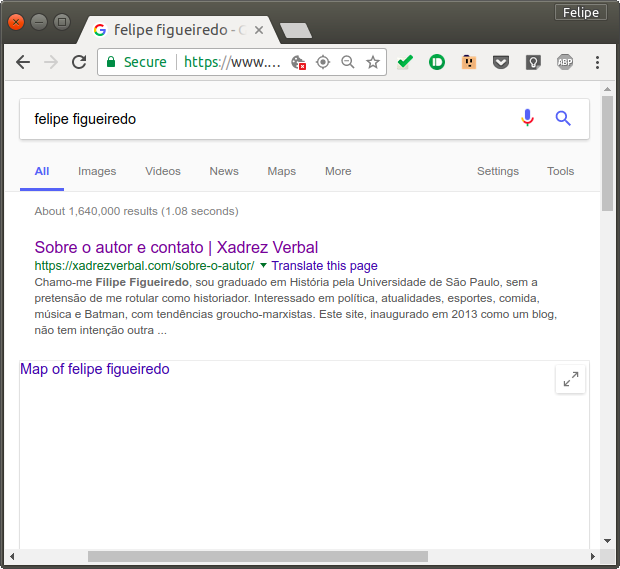
\includegraphics[height=.7\textheight]{Cap1/felipefigueiredo-not1}
    \begin{exampleblock}{}
      \begin{center}
        \footnotesize
        {\bf Não sou Historiador}
      \end{center}
    \end{exampleblock}
  \end{center}
\end{frame}

\begin{frame}{\scriptsize Google: dr felipe figueiredo}
  \begin{center}
    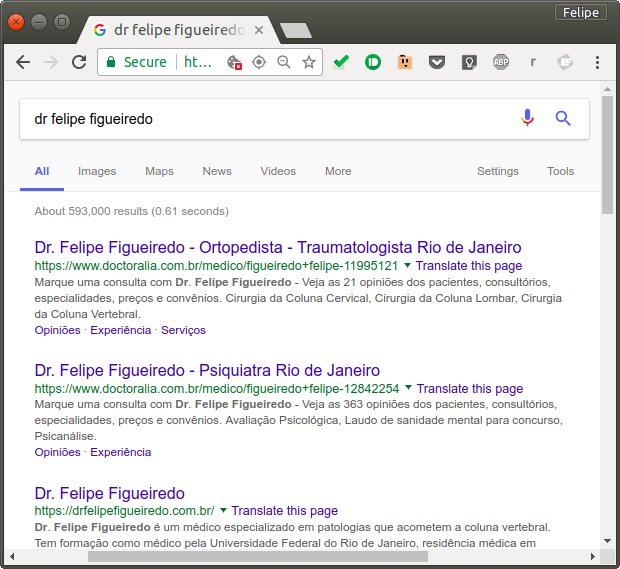
\includegraphics[height=.7\textheight]{Cap1/felipefigueiredo-not2}
    \begin{exampleblock}{}
      \begin{center}
        \footnotesize
        {\bf Não sou Psiquiatra ou Ortopedista}
      \end{center}
    \end{exampleblock}
  \end{center}
\end{frame}

\begin{frame}{\scriptsize Google: prof felipe figueiredo}
  \begin{center}
    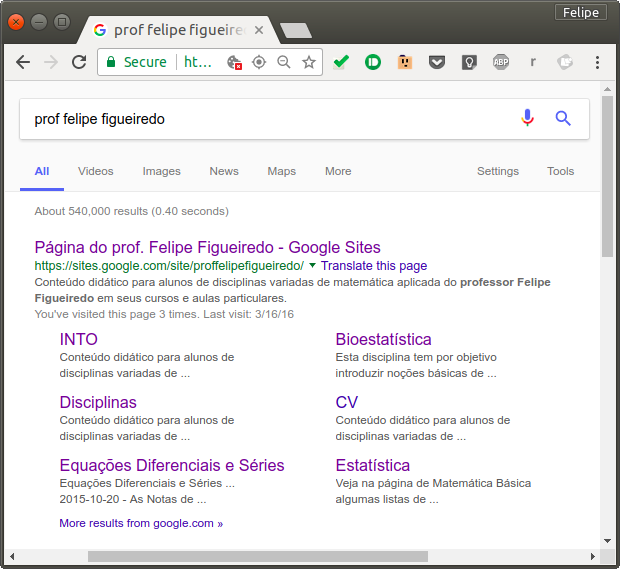
\includegraphics[height=.7\textheight]{Cap1/felipefigueiredo}
    \begin{exampleblock}{}
      \begin{center}
        \footnotesize
        Este que vos fala, a seu dispor.
      \end{center}
    \end{exampleblock}
  \end{center}
\end{frame}

\begin{frame}{\scriptsize Objetivos de aprendizagem}
  \begin{block}{}
    \footnotesize
    Interpretar criticamente dados e resultados de artigos científicos.
  \end{block}
  \begin{block}{}
    \footnotesize
    Adquirir autonomia nas análises estatísticas em nível de mestrado.
  \end{block}
\end{frame}

\subsection{Disciplina moderna, material online}

% \begin{frame}{Avaliação}
%   \begin{itemize}
%   \item {\bf Objetivo:} interpretar criticamente um paper
%   \item Seminário (grupo)
%   \item Dois últimos encontros
%   \item Roteiro disponível para auxiliar a elaboração.
%   \end{itemize}
% \end{frame}

\begin{frame}{\scriptsize Bibliografia}
  \begin{block}{Livro texto}
    \footnotesize
    MOTULSKY, H. (1995) {\em Intuitive Biostatistics}, 1 ed.
  \end{block}
  \bigskip
  \begin{itemize}
    \scriptsize
  \item Alguns capítulos (última edição) disponíveis gratuitamente no site da editora;
  \item Fontes de apoio online (apostilas e papers).
  \end{itemize}
\end{frame}

\begin{frame}{\scriptsize Material online}
  \footnotesize
  Todas as informações, avisos, aulas, etc. serão disponibilizados online
  \begin{block}{Site (http / https)}
    \footnotesize
    \url{sites.google.com/site/proffelipefigueiredo/}
  \end{block}
  % Adicionalmente, avisos importantes podem ser divulgados no blog
  % \begin{block}{Blog}
  %   \small
  %   \url{http://proffelipefigueiredo.blogspot.com.br/}
  % \end{block}

  \bigskip
  O endereço não é de fácil memorização, portanto uma busca no Google é o melhor caminho.

  \bigskip
  Você pode procurar pelo meu nome (Felipe Figueiredo)

  \bigskip
  \bigskip
  Porém...
\end{frame}

\begin{frame}{\scriptsize Bem vindos ao séc. XXI}
  \begin{block}{Gestão da disciplina}
    \footnotesize
    Estamos migrando do formato de uma página fixa da disciplina, para uma plataforma dinâmica.
  \end{block}
  \begin{itemize}
    \footnotesize
  \item Endereço da página da disciplina

    \url{https://sites.google.com/site/proffelipefigueiredo/into/bioestatistica}
  \end{itemize}
  \begin{block}{Nova plataforma: Google Sala de Aula}
    \footnotesize
    Instale agora no seu celular/tablet o app

    \bigskip
    {\bf Google Sala de Aula}
  \end{block}
\end{frame}

\begin{frame}{\scriptsize Google Sala de Aula apps (iOS e Android)}
  \begin{center}
    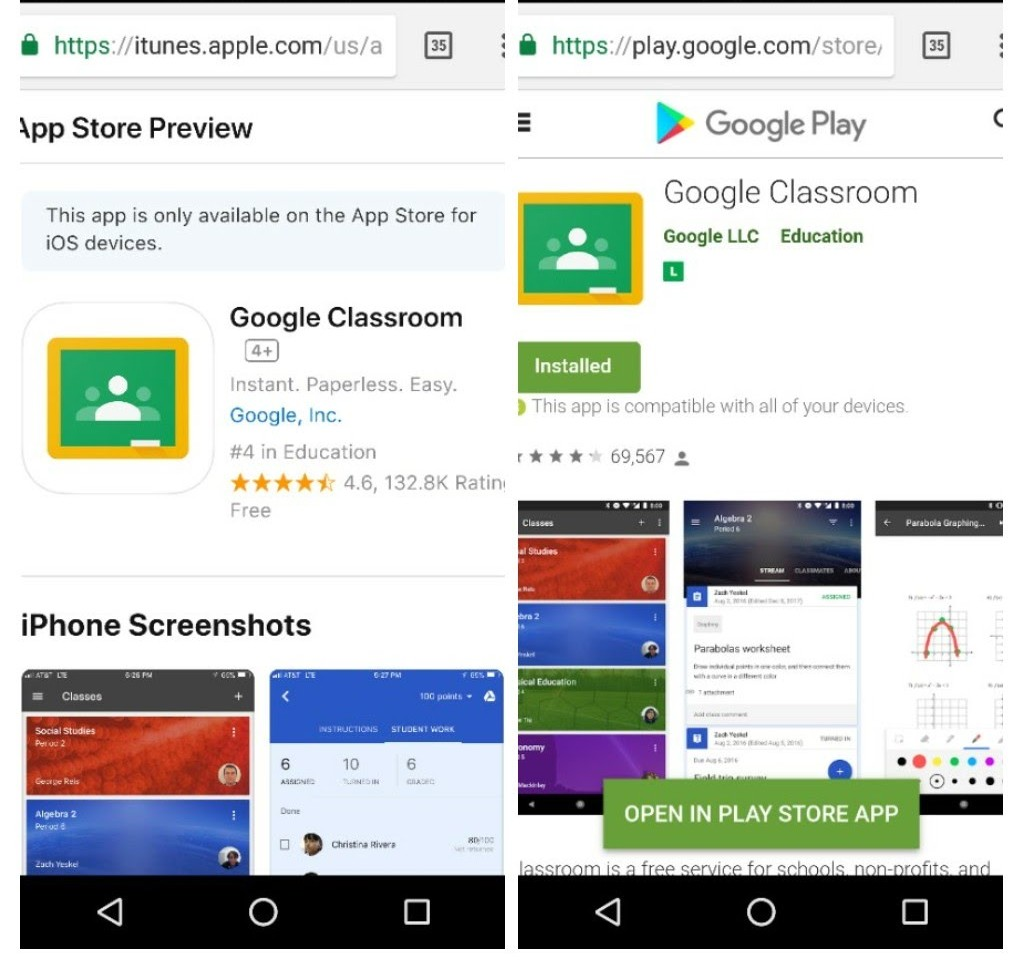
\includegraphics[height=\textheight]{Cap1/gclassroom-apps}
  \end{center}
\end{frame}

\begin{frame}{\scriptsize Clique no + e digite o código da turma}
  \begin{center}
    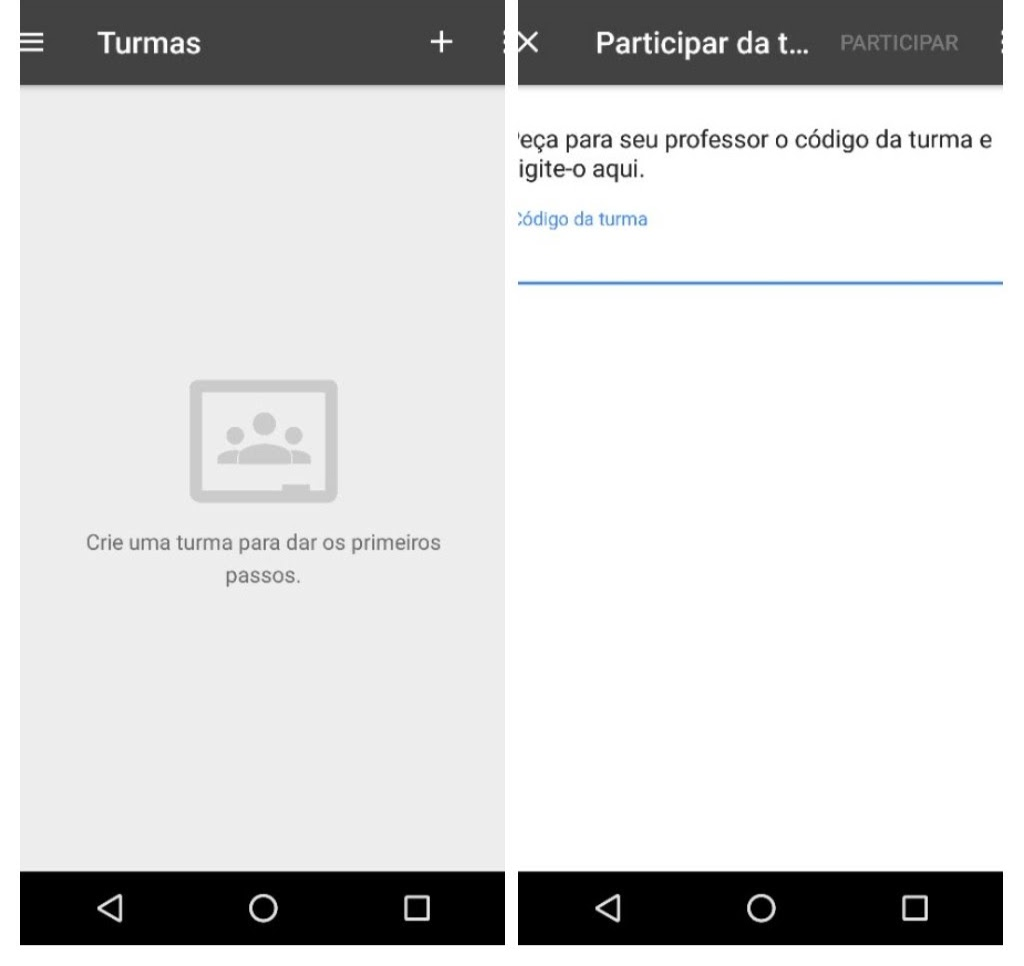
\includegraphics[height=\textheight]{Cap1/gclassroom-turma}
  \end{center}
\end{frame}

\begin{frame}{\scriptsize Google Sala de Aula}
  \begin{itemize}
    \footnotesize
  \item Tarefas por assuntos, pré aula e pós aula
  \item Prazos
  \item A primeira: ambientação com a plataforma
  \item Prazos\footnote{Você já está devendo tarefas}
  \end{itemize}
\end{frame}

\section{Bioestatística}

\subsection{Cap 1: Bioestatística é difícil}

\begin{frame}{\scriptsize Bioestatística é difícil}
  \begin{enumerate}
    \footnotesize
  \item Terminologia conflita com termos usuais
  \item ``Estatisticamente significante'' tem apelo mágico
  \item Conceitos abstratos
  \item Interface entre a Ciência e a Matemática
  \item Não costuma ser Matemática básica
  \end{enumerate}
\end{frame}

\subsection{Aspectos gerais}

\begin{frame}{\scriptsize O que é}
  \begin{columns}
    \begin{column}{7cm}
      \begin{block}{}
        {\scriptsize ``{\em The Statistician is the Wizard who makes
            `scientific' statements about invisible states and
            quantities. However, contrary to the real wishes (or
            witches), he attaches uncertainties to his statements}'' –
          Carlos A.  Pereira.}
      \end{block}
      \begin{block}{}
        {\scriptsize ``{\em Se você torturar os dados o suficiente,
            eles confessarão o que você quiser.}'' - Ronald H. Coase}
      \end{block}

    \end{column}
    \begin{column}{3cm}
      \begin{center}
        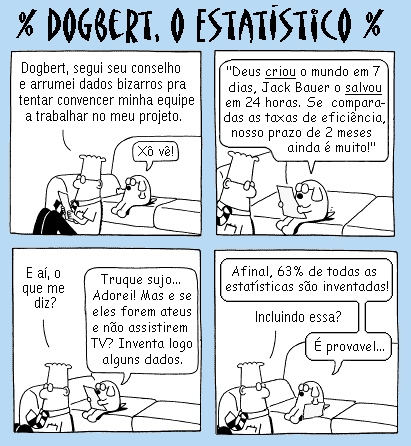
\includegraphics[width=1.6\textwidth]{Cap1/dilbert}
      \end{center}
    \end{column}
  \end{columns}
\end{frame}

\begin{frame}{\scriptsize Método Científico}
  \begin{enumerate}
    \footnotesize
  \item Observação do fenômeno (problema)
  \item Formulação de uma hipótese
  \item Experimento
  \item Validação ou refutação da hipótese
  \end{enumerate}
\end{frame}

\begin{frame}{\scriptsize Método Científico}
  \begin{itemize}
    \footnotesize
  \item Experimentos tem incertezas
    \begin{itemize}
      \scriptsize
    \item Coleta de dados imperfeita
    \item Incompletude dos dados
    \item Erros de medição
    \item Formulação incompleta de hipóteses
    \end{itemize}
  \end{itemize}
\end{frame}

\begin{frame}{\scriptsize Método Estatístico}
  \begin{itemize}
    \footnotesize
  \item Como extrair informação a partir dos dados?
  \item Como lidar com as incertezas?
  \end{itemize}

  \begin{center}
    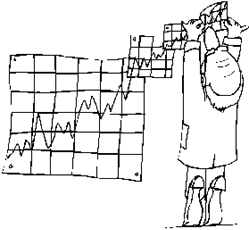
\includegraphics[height=.4\textheight]{Cap1/Probabilidades}
  \end{center}
\end{frame}

% \begin{frame}{Método Estatístico}
%   \begin{enumerate}
%   \item Planejamento do experimento
%   \item Coleta/aquisição dos dados
%   \item Organização e descrição dos dados
%   \item Análise/interpretação
%   \item Informação/tomada de decisão
%   \end{enumerate}
% \end{frame}

\begin{frame}{\scriptsize Para que serve}
  \begin{itemize}
    \footnotesize
  \item Desnecessária: diferenças muito grandes
  \item Necessária: detectar diferenças pequenas
  \item Necessária: detectar diferenças, quando há muita variabilidade nos dados
  \end{itemize}
\end{frame}

% \begin{frame}{Áreas da Estatística}
%   \begin{itemize}
%   \item Análise Descritiva
%   \item Probabilidade
%   \item Inferência
%   \item Modelagem
%   \end{itemize}
% \end{frame}

\begin{frame}{\scriptsize Para que serve}
  \begin{itemize}
    \footnotesize
  \item Modelos explanatórios
  \item Modelos preditivos
  \end{itemize}
\end{frame}

\begin{frame}{\scriptsize O que você vai aprender}
  \begin{center}
    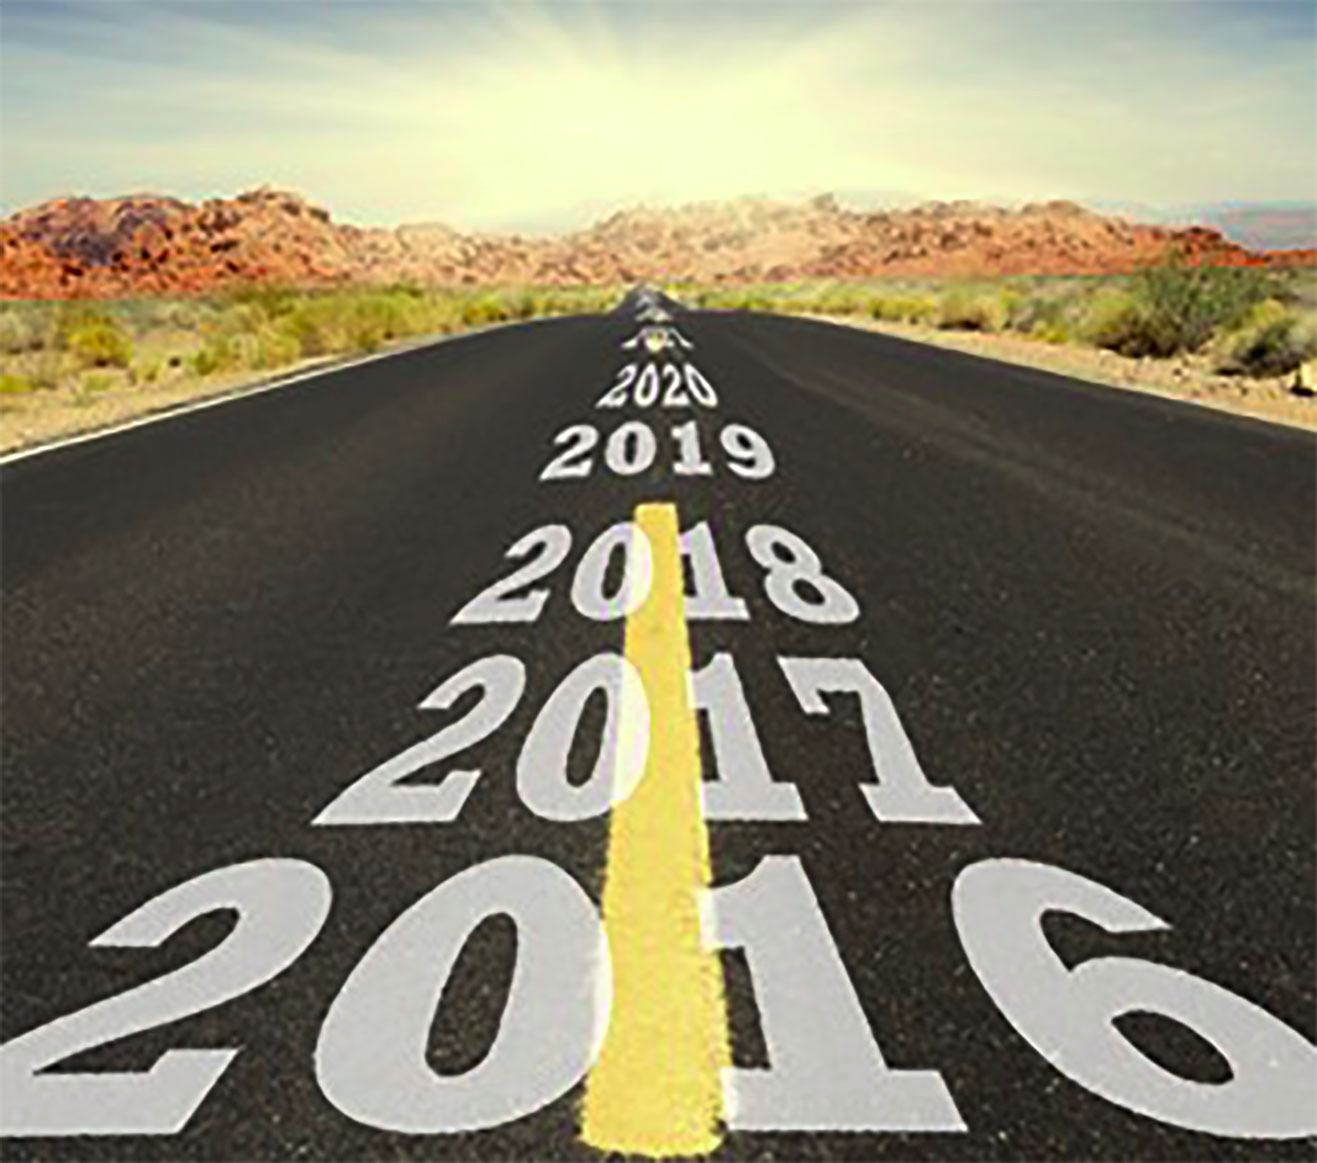
\includegraphics[height=\textheight]{Cap1/road-ahead}
  \end{center}
\end{frame}

\begin{frame}{\scriptsize O que você vai aprender}
  \footnotesize
  Você vai entender esse gráfico

  \bigskip
  \begin{center}
    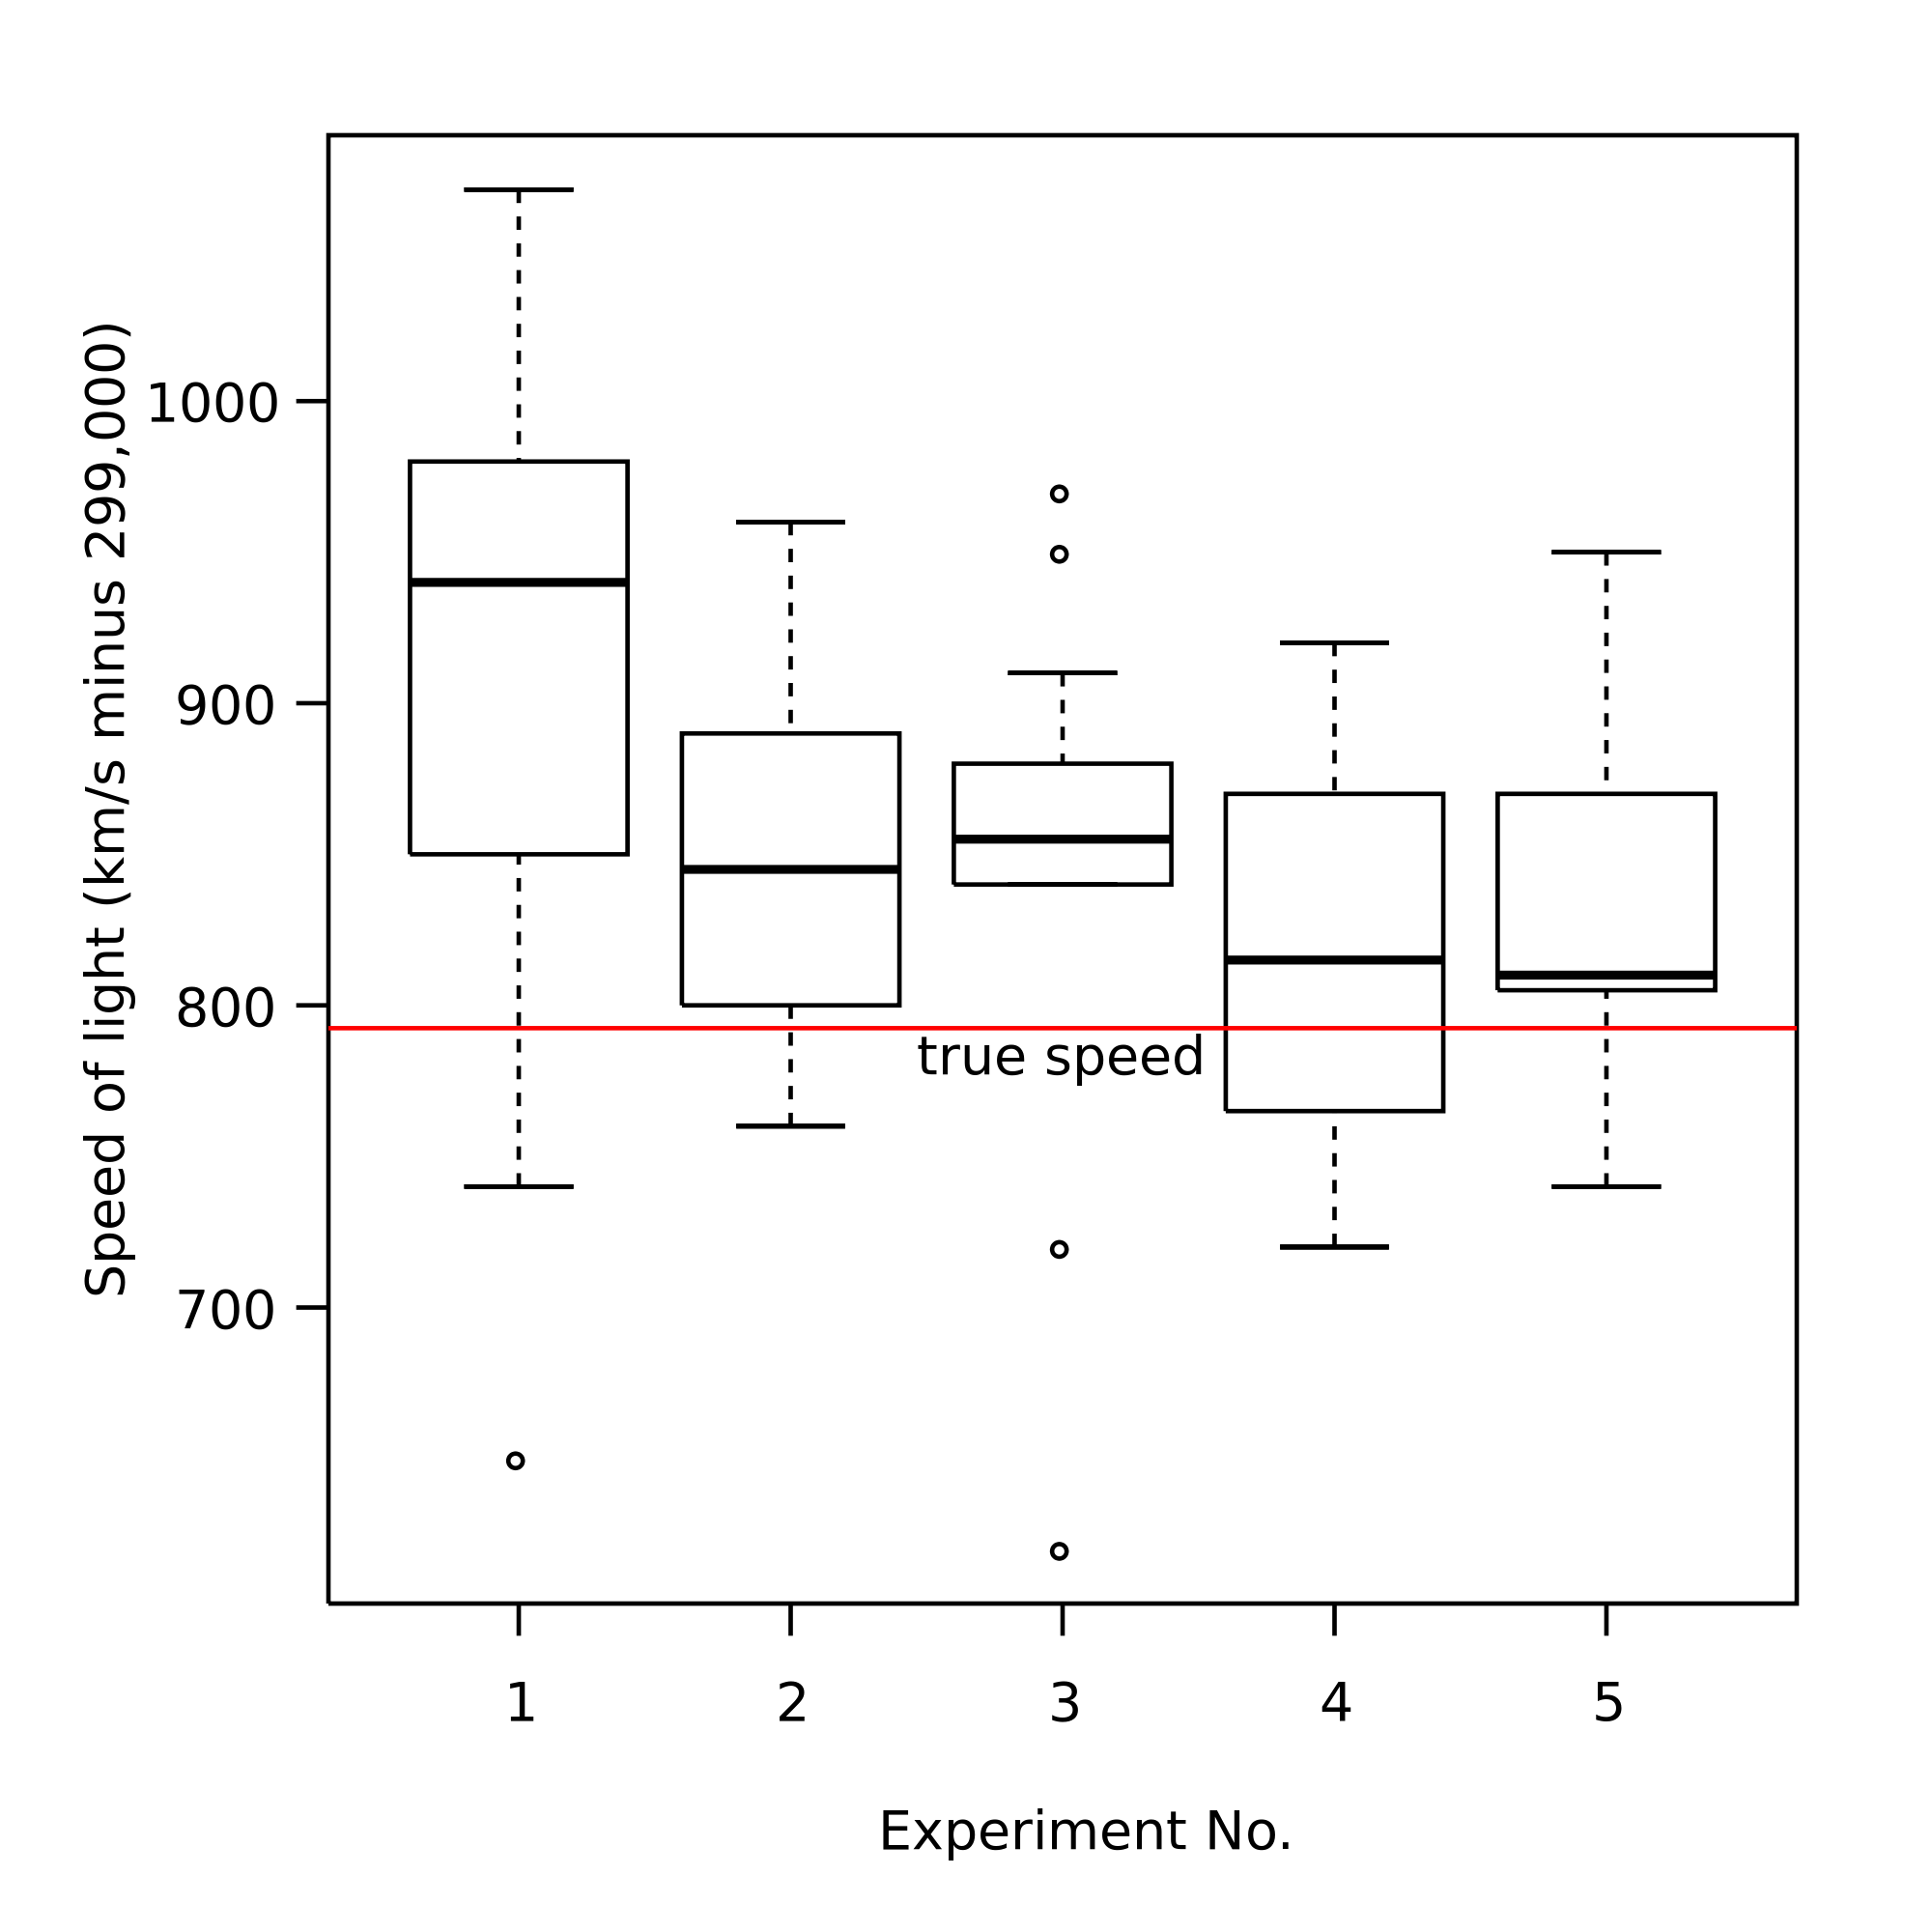
\includegraphics[width=.65\textwidth]{Cap1/boxplot}
  \end{center}
\end{frame}

\begin{frame}{\scriptsize O que você vai aprender}
  \footnotesize
  Você vai entender esse gráfico

  \bigskip
  \begin{center}
    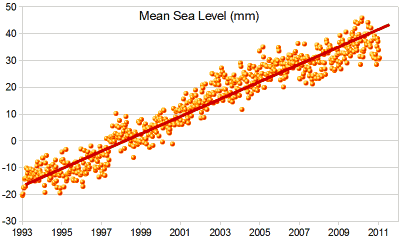
\includegraphics[width=.7\textwidth]{Cap1/mean-sea-level-line}
  \end{center}
\end{frame}

\begin{frame}{\scriptsize O que você vai aprender}
  \footnotesize
  Você vai entender a diferença entre esses gráficos

  \bigskip
  \begin{center}
    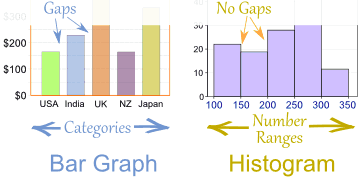
\includegraphics[width=.7\textwidth]{Cap1/bar-chart-vs-histogram}
  \end{center}
\end{frame}

\begin{frame}{\scriptsize mas não é só isso}
  \begin{center}
    
\includegraphics[width=.7\textwidth]{Cap1/bottini}
  \end{center}
\end{frame}

\begin{frame}{\scriptsize O que você vai aprender}
  \begin{block}{}
    \footnotesize
    Você ficaria surpreso(a) que pode aprender a pensar desta forma?
  \end{block}

  $$\text{var. dependente} \sim \text{var. independente} + \varepsilon$$
\end{frame}

\begin{frame}{\scriptsize O que você vai aprender}
  \begin{block}{}
    \footnotesize
    Você ficaria surpreso(a) que pode aprender a pensar desta forma?
  \end{block}

  $$\text{desfecho} \sim \text{preditor} + \varepsilon$$
\end{frame}

\begin{frame}{\scriptsize }
  \begin{exampleblock}{Exemplo 1}
    \footnotesize
    Você quer dosar a proteína C reativa em
    \begin{itemize}
    \footnotesize
    \item um grupo de tratamento
    \item um grupo controle
    \end{itemize}
    e comparar as mensurações deste grupo com as mensurações dos grupos.
  \end{exampleblock}
  \begin{block}{Pergunta}
    \footnotesize
    Quantas e quais variáveis estão consideradas?
  \end{block}
\end{frame}

\begin{frame}{\scriptsize }
  \begin{exampleblock}{Exemplo 2}
    \footnotesize
    Você quer dosar a proteína C reativa em
    \begin{itemize}
    \footnotesize
    \item um grupo com uma dieta nutricional específica
    \item um grupo com um medicamento
    \item um grupo com ambas as opções acima
    \item um grupo controle
    \end{itemize}
    e comparar as mensurações deste grupo com as mensurações dos grupos.
  \end{exampleblock}
  \begin{block}{Pergunta}
    \footnotesize
    Quantas e quais variáveis estão consideradas?
  \end{block}
\end{frame}

\begin{frame}{\scriptsize O que você vai aprender}
  \begin{block}{}
    \footnotesize
    Você ficaria surpreso(a) que pode aprender a pensar desta forma?
  \end{block}

  $$\text{PCR} \sim \text{grupo} + \text{erro}$$
\end{frame}

\begin{frame}{\scriptsize Em outro momento...}
  \begin{block}{}
    \footnotesize
    Você pode incorporar outros detalhes
  \end{block}

  $$\text{PCR} \sim \text{grupo} + \text{fator de exposição} + \text{erro}$$
\end{frame}

\begin{frame}{\scriptsize Para isto}
  \begin{itemize}
    \footnotesize
  \item Aulas expositivas
  \item Leitura pós aula (obrigatória e recomendada)
  \item Exercícios de fixação (do livro)
  \item Tarefas pós aula (interpretação de conceitos)
  \item Tarefas pré aula
  \item ... e muito mais!
  \end{itemize}
\end{frame}

\begin{frame}{\scriptsize Resumindo}
  \begin{itemize}
    \footnotesize
  \item Computadores fazem cálculos melhor que nós
  \item A disciplina {\bf não} foca nos cálculos
    \begin{itemize}
    \item exposição de fórmulas $\Rightarrow$ fatores relevantes
    \end{itemize}
  \item Você deve aprender a interpretar resultados
  \end{itemize}
\end{frame}

% \section{Trailer do curso}

% \begin{frame}{\scriptsize Dados}
%   \begin{itemize}
%   \item Qualitativos (contagens/proporções)
%   \item Quantitativos (medidas/mensurações)
%   \end{itemize}
% \end{frame}

% \begin{frame}{\scriptsize Tipos de Dados}
% Dados podem ser classificadas em duas principais categorias
%   \begin{itemize}
%   \item Qualitativos (categóricos)
%   \item Quantitativos (numéricos)
%   \end{itemize}
%   \begin{example}
%     Pressão sistólica (mmHg), altura (cm), sexo (M ou F), grau de
%     satisfação com atendimento médico (escore de 1 a 5), perímetro
%     abdominal (cm), contagem de leucócitos, número de pessoas na
%     família, cor da pele (branco, negro, pardo), etc.
%   \end{example}
% \end{frame}

% \begin{frame}{\scriptsize Descrição dos Dados}
%   \begin{itemize}
%   \item Organização/visualização
%     \begin{itemize}
%     \item Tabelas
%     \item Gráficos
%     \end{itemize}
%   \item Medidas sumárias
%     \begin{itemize}
%     \item Medidas de tendência central
%     \item Medidas de dispersão
%     \end{itemize}
%   \end{itemize}
% \end{frame}

% \begin{frame}{\scriptsize Trailer do curso}
%   \begin{columns}
%     \begin{column}{5cm}
%       \begin{center}
%         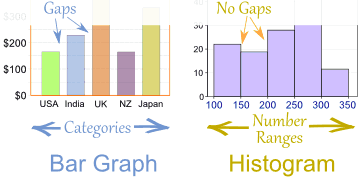
\includegraphics[width=.9\textwidth]{Cap1/bar-chart-vs-histogram}

%       \bigskip
%       \bigskip
%       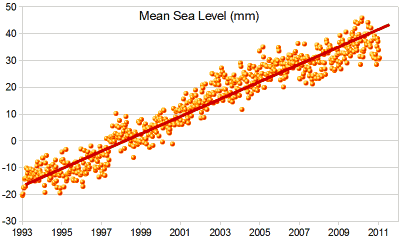
\includegraphics[width=.9\textwidth]{Cap1/mean-sea-level-line}
%       \end{center}
%     \end{column}
%     \begin{column}{6cm}
%       \begin{center}
%         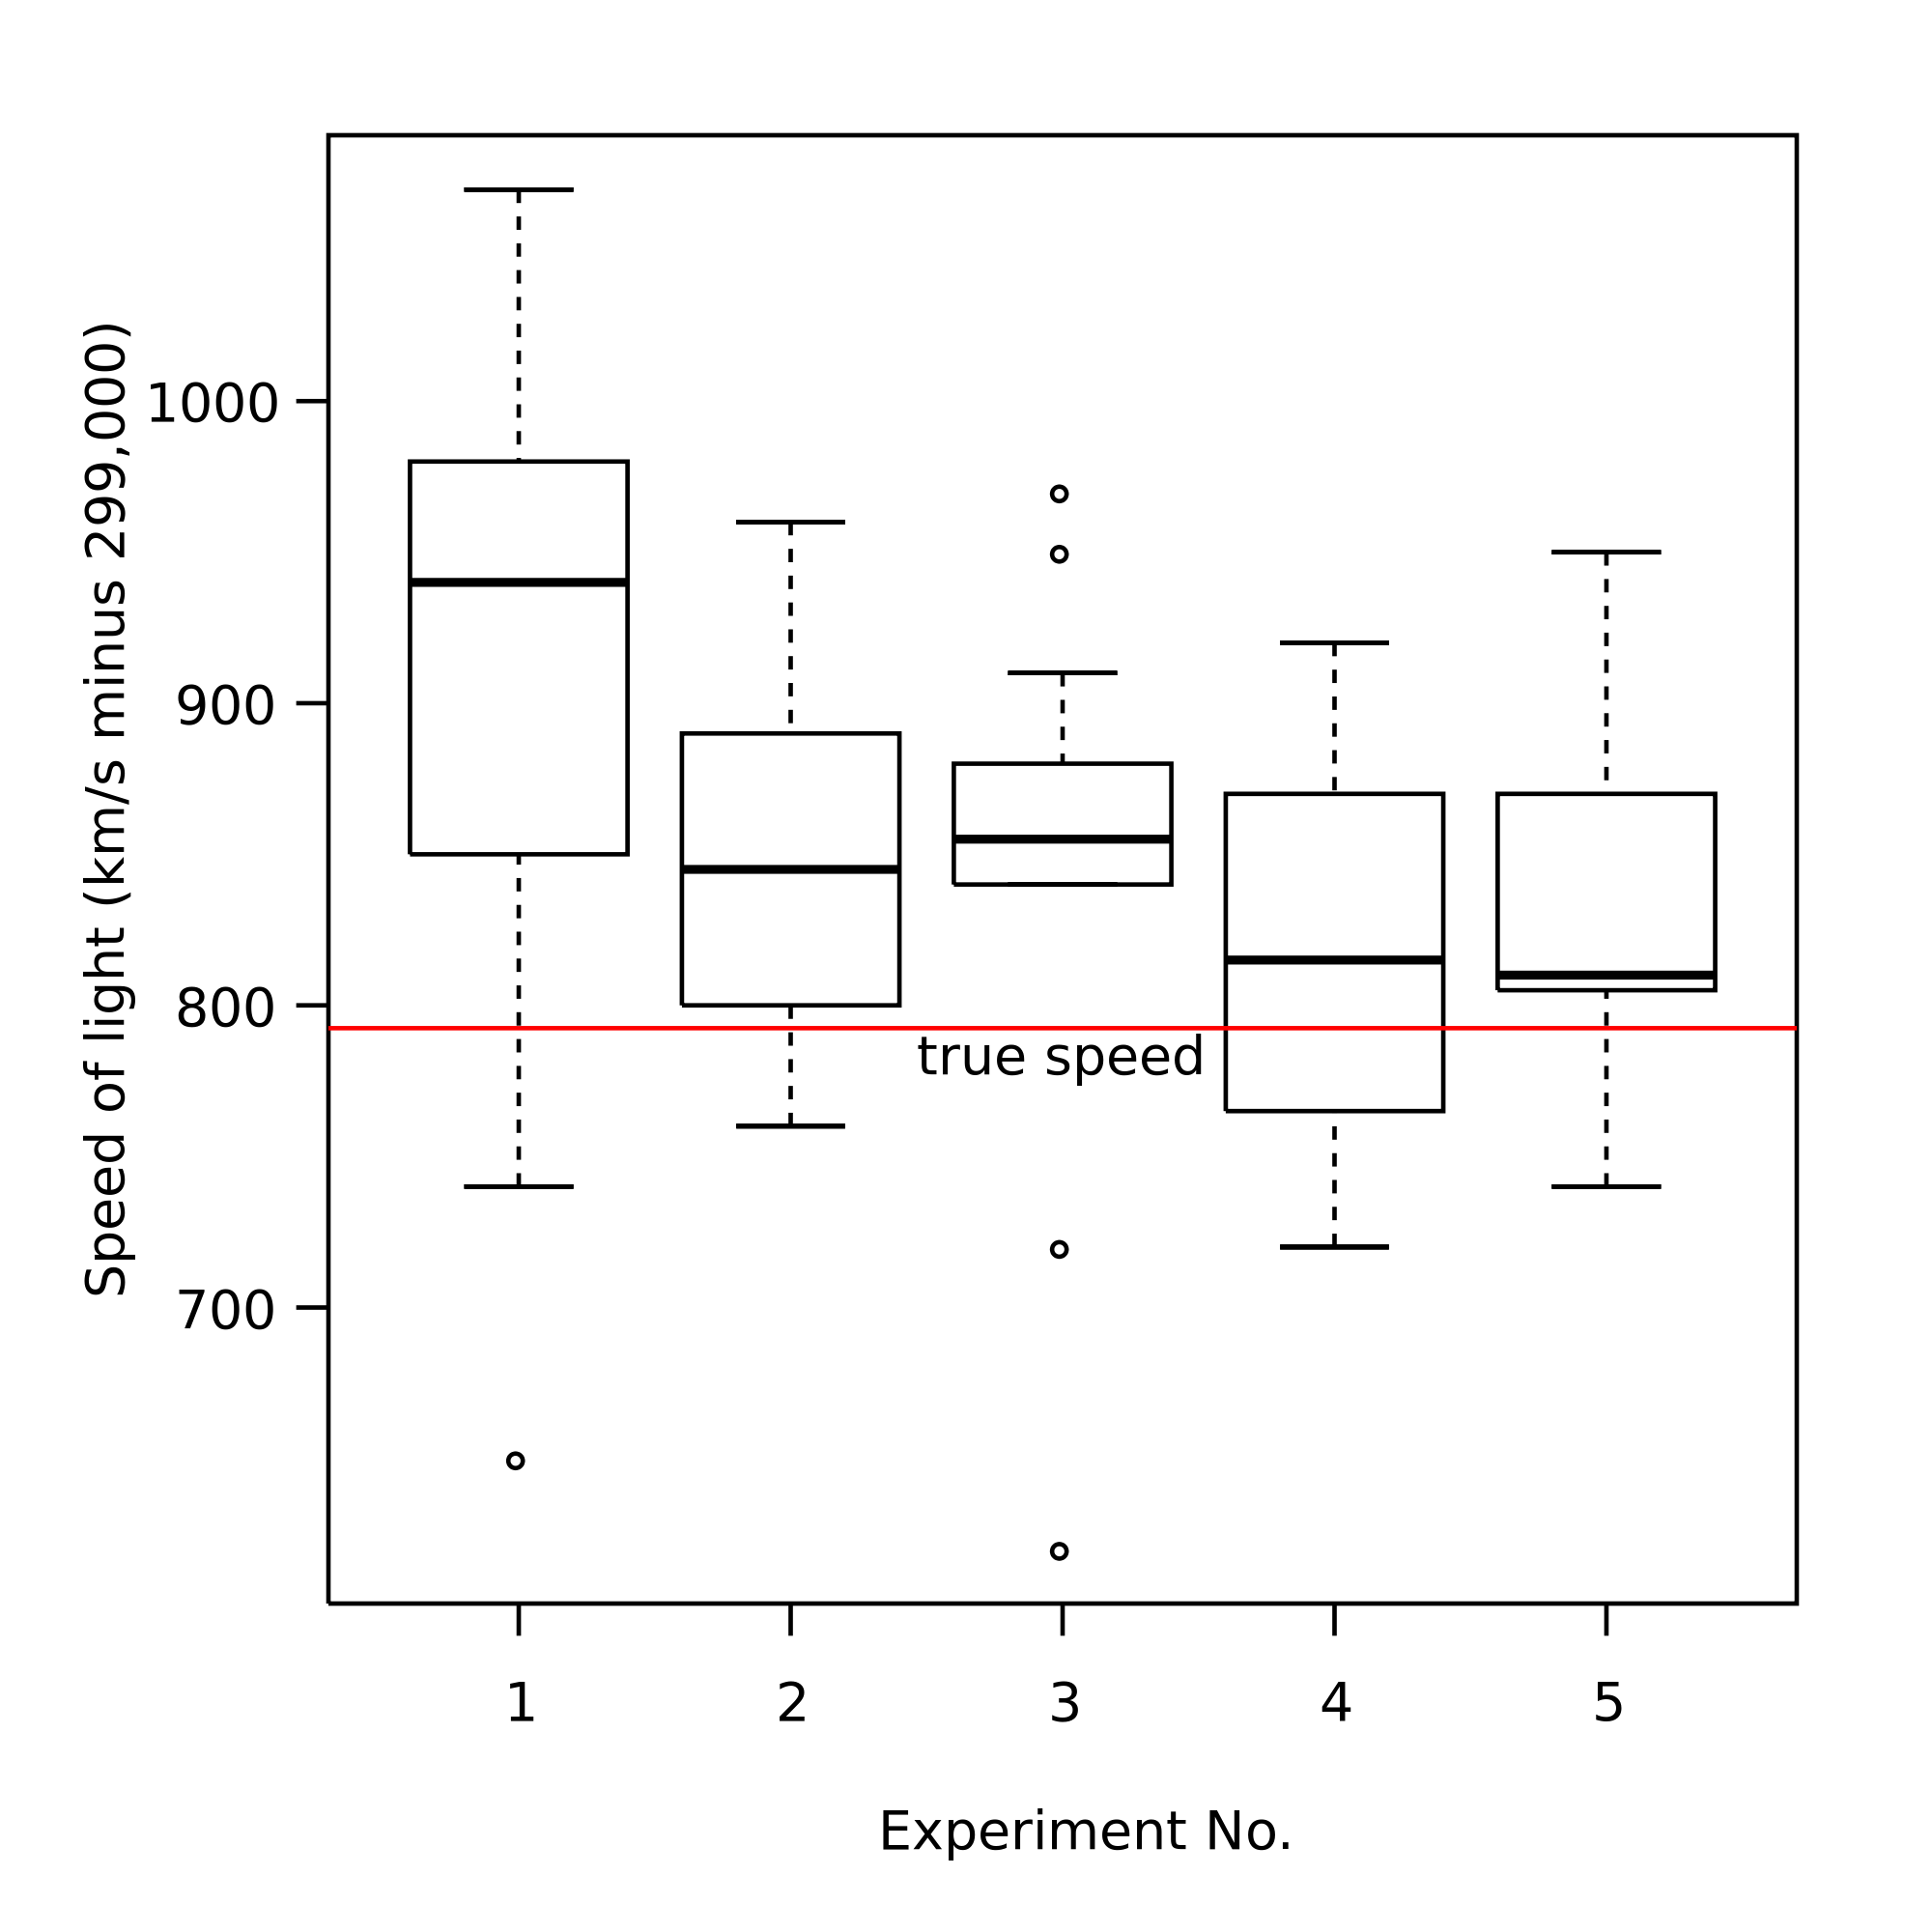
\includegraphics[width=.7\textwidth]{Cap1/boxplot}

%       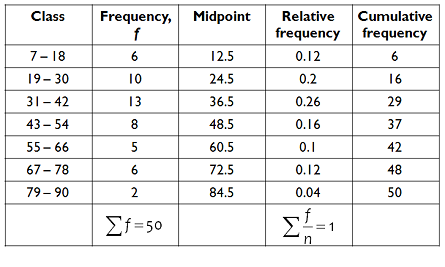
\includegraphics[width=.9\textwidth]{Cap1/table}
% %[height=.5\textheight]
%       \end{center}
%     \end{column}
%   \end{columns}
% \end{frame}

% \begin{frame}{\scriptsize Trailer do curso}
% Vamos fazer um pequeno experimento didático

%   \begin{block}{Dados necessários}
%     \begin{itemize}
%     \item Sexo
%     \item Altura (cm)
%     \item Tamanho do sapato
%     \end{itemize}
%   \end{block}
% \end{frame}

\subsection{Aprofundamento}

\begin{frame}{\scriptsize Aprofundamento}
  \begin{block}{Pós aula}
    \footnotesize
    Livro texto: Cap {\bf 1}
  \end{block}
  % \begin{block}{Pré aula (semana que vem)}
  %   \footnotesize
  %   Tarefas no Google Sala de Aula (artigo e atividade básica)
  % \end{block}
  \begin{block}{Leitura recomendada}
    \footnotesize
    Livro texto: Cap {\bf 2} (passar os olhos)
  \end{block}
\end{frame}

\end{document}
